\documentclass[sigconf, review]{acmart}

\usepackage[outline]{contour}
\usepackage{invariantconfluence}
\usepackage{pervasives}
\usepackage{subcaption}
\usepackage{tikz}
\usetikzlibrary{arrows}

% Copyright
%\setcopyright{none}
%\setcopyright{acmcopyright}
%\setcopyright{acmlicensed}
\setcopyright{rightsretained}
%\setcopyright{usgov}
%\setcopyright{usgovmixed}
%\setcopyright{cagov}
%\setcopyright{cagovmixed}

% DOI
\acmDOI{10.475/123_4}

% ISBN
\acmISBN{123-4567-24-567/08/06}

%Conference
\acmConference[WOODSTOCK'97]{ACM Woodstock conference}
                            {July 1997}
                            {El Paso, Texas USA}
\acmYear{1997}
\copyrightyear{2016}
\acmArticle{4}
\acmPrice{15.00}

\begin{document}
\title{TODO}
% \title{A Confluence of Ideas:\\Determining when Weak Consistency is Good Enough}
% \title{In the Sky with Diamonds:\\Determining when Weak Consistency is Good Enough}
% \title{A Confluence of Ideas:\\Maintaining Invariants of Distributed Data}
% \title{In the Sky with Diamonds:\\Maintaining Invariants of Distributed Data}
% \title{Coordination Freedom, Strong Invariants: Pick Two}

\author{Michael Whittaker}
\affiliation{%
  \institution{UC Berkeley}
}
\email{mjwhittaker@berkeley.edu}

\author{Joseph M. Hellerstein}
\affiliation{%
  \institution{UC Berkeley}
}
\email{hellerstein@berkeley.edu}

{\begin{abstract}
Strongly consistent systems are easy to reason about but face fundamental
limitations in availability and performance. Weakly consistent systems can be
implemented with very high performance but place a burden on the application
developer to reason about complex interleavings of execution.
\Invariantconfluence{} provides a formal framework for understanding when we
can get the best of both worlds. An \invariantconfluent{} object can be
efficiently replicated with no coordination needed to preserve its invariants.
However, actually determining whether or not an object is \invariantconfluent{}
is challenging: undecidable in general. In this paper, we establish conditions under
which a commonly used sufficient condition for \invariantconfluence{} is both
necessary and sufficient and use this condition to design (a) a general-purpose
interactive \invariantconfluence{} decision procedure and (b) a novel
sufficient condition that can be checked automatically. We then take a step
beyond \invariantconfluence{} and introduce a generalization of
\invariantconfluence{} called segmented \invariantconfluence{}, which allows us
to replicate non-\invariantconfluent{} objects with a small amount of
coordination. We implemented our theoretical findings in a prototype called
Lucy and found that our decision procedures efficiently handle common real-world workloads
including foreign key constraints, rollups, escrow transactions, and others.  We also
found that segmented \invariantconfluent{} replication can deliver up to an
order of magnitude more throughput than linearizable replication for low
contention workloads and comparable throughput for medium to high contention
workloads.
\end{abstract}
}

% The code below should be generated by the tool at
% http://dl.acm.org/ccs.cfm
% Please copy and paste the code instead of the example below.
\begin{CCSXML}
<ccs2012>
 <concept>
  <concept_id>10010520.10010553.10010562</concept_id>
  <concept_desc>Computer systems organization~Embedded systems</concept_desc>
  <concept_significance>500</concept_significance>
 </concept>
 <concept>
  <concept_id>10010520.10010575.10010755</concept_id> <concept_desc>Computer systems organization~Redundancy</concept_desc>
  <concept_significance>300</concept_significance>
 </concept>
 <concept>
  <concept_id>10010520.10010553.10010554</concept_id>
  <concept_desc>Computer systems organization~Robotics</concept_desc>
  <concept_significance>100</concept_significance>
 </concept>
 <concept>
  <concept_id>10003033.10003083.10003095</concept_id>
  <concept_desc>Networks~Network reliability</concept_desc>
  <concept_significance>100</concept_significance>
 </concept>
</ccs2012>
\end{CCSXML}

\ccsdesc[500]{Computer systems organization~Embedded systems}
\ccsdesc[300]{Computer systems organization~Redundancy}
\ccsdesc{Computer systems organization~Robotics}
\ccsdesc[100]{Networks~Network reliability}

\keywords{ACM proceedings, \LaTeX, text tagging}

\maketitle
{\section{Introduction}
When an application designer decides to replicate a piece of data, they have to
make a fundamental choice between weak and strong consistency. Replicating the
data with strong consistency using a technique like distributed transactions
(e.g.,~\cite{bernstein1981concurrency,mohan1986transaction}) or state machine
replication (e.g.,~\cite{schneider1990implementing, lamport1998part,
liskov2012viewstamped, ongaro2014search}) makes the application designer's life
very easy. To the developer, a strongly consistent system behaves exactly like
a single-threaded system running on a single node, so reasoning about the
behavior of the system is simple~\cite{herlihy1990linearizability}.
Unfortunately, strong consistency is at odds with performance. The CAP theorem
and PACELC theorem tell us that strongly consistent systems suffer from higher
latency at best and unavailability at worst~\cite{gilbert2002brewer,
brewer2012cap, abadi2012consistency}. On the other hand, weak consistency
models like eventual consistency~\cite{vogels2009eventually}, PRAM
consistency~\cite{lipton1988pram}, causal consistency~\cite{ahamad1995causal},
and others~\cite{lloyd2011don, mehdi2017can} allow data to be replicated with
high availability and low latency, but they put a tremendous burden on the
application designer to reason about the complex interleavings of operations
that are allowed by these weak consistency models. In particular, weak
consistency models strip an application developer of one of the earliest and
most effective tools that is used to reason about the execution of programs:
application invariants~\cite{hoare1969axiomatic, balegas2015towards} such as
database integrity constraints~\cite{grefen1993integrity, gupta1993local}. Even
if every transaction executing in a weakly consistent system individually
maintains an application invariant, the system as a whole can produce
invariant-violating states.

Is it possible for us to have our strongly consistent cake and eat it with high
availability too? Can we replicate a piece of data with weak consistency but
still ensure that its invariants are maintained? Yes... sometimes. Bailis et
al.\ introduced the notion of \emph{\invariantconfluence{}} as a necessary and
sufficient condition for when invariants can be maintained over replicated data
without the need for any coordination~\cite{bailis2014coordination}. If an
object is \invariantconfluent{} with respect to an invariant, we can replicate
it with the performance benefits of weak consistency and (some of) the
correctness benefits of strong consistency.

Unfortunately, to date, the task of identifying whether or not an object
actually is \invariantconfluent{} has remained an exercise in human proof
generation. Bailis et al.\ manually categorized a set of common objects,
transactions, and invariants (e.g.\ foreign key constraints on relations,
linear constraints on integers) as \invariantconfluent{} or not. Hand-written
proofs of this sort are unreasonable to expect from programmers. Ideally we
would have a general-purpose program that can automatically determine
\invariantconfluence{} for us.  \textbf{The first main thrust of this paper is
to make \invariantconfluence{} checkable:} to design a general-purpose
\invariantconfluence{} decision procedure, and implement it in an interactive
system.

Unfortunately, designing such a general-purpose decision procedure is
impossible because determining the \invariantconfluence{} of an object is
undecidable in general. Still, we can develop a decision procedure that works
well in the common case.
%
For example, many prior efforts have developed decision procedures for
\emph{\invariantclosure{}}, a sufficient (but not necessary) condition for
\invariantconfluence{}~\cite{li2012making, li2014automating}. The existing
approaches check whether an object is \invariantclosed{}. If it is, then they
conclude that it is also \invariantconfluent{}. If it's not, then the current
approaches are unable to conclude anything about whether or not the object is
\invariantconfluent{}.

In this paper, we take a step back and study the underlying reason \emph{why}
\invariantclosure{} is not necessary for \invariantconfluence{}.
%
% We find that \invariantconfluence{} is fundamentally a reachability property,
% checking whether certain values of our replicated object can actually be
% obtained in the execution of a system. We discover that unreachable, yet
% invariant satisfying, states cause \invariantclosure{} to be an unnecessary
% condition.
%
Using this understanding, we construct a set of modest conditions under which
\invariantclosure{} and \invariantconfluence{} are in fact \emph{equivalent},
allowing us to reduce the problem of determining \invariantconfluence{} to that
of determining \invariantclosure{}.
%
Then, we use these conditions to design a general-purpose interactive
\invariantconfluence{} decision procedure and a new sufficient condition for
\invariantconfluence{}, dubbed \emph{\mergereducibility}. \Mergereducibility{}
covers some cases that are not covered by \invariantclosure{}, and it can be
checked automatically.

% Then, we use these conditions to design a general-purpose interactive
% \invariantconfluence{} decision procedure. Users iteratively interact with the
% decision procedure, eliminating unreachable states from the invariant, moving
% towards the conditions under which \invariantclosure{} and
% \invariantconfluence{} are equivalent. Meanwhile, the decision procedure
% generates examples of reachable and unreachable states which help the user
% recognize patterns that describe reachability. We also leverage our intuitions
% about reachability to develop a new sufficient condition for
% \invariantconfluence{}, dubbed \emph{\mergereducibility}. \Mergereducibility{}
% covers some cases that are not covered by \invariantclosure{}, and it can be
% automatically checked without any user interaction.

\textbf{The second main thrust of this paper is to partially avoid coordination
even in programs that require it}, by generalizing \invariantconfluence{} to a
property called \emph{segmented \invariantconfluence{}}. While
\invariantconfluence{} characterizes objects that can be replicated
\emph{without any} coordination, segmented \invariantconfluence{} allows us to
replicate non-\invariantconfluent{} objects with only \emph{occasional}
coordination. The main idea is to divide the set of invariant-satisfying states
into \emph{segments}, with a restricted set of transactions allowed in each
segment.  Within a segment servers act without any coordination; they
synchronize only to transition across segment boundaries. This design
highlights the trade-off between application complexity and
coordination-freedom; more complex applications require more segments which
require more coordination, and vice-versa.

Finally, we present Lucy: an implementation of our decision procedures and a
system for replicating \invariantconfluent{} and segmented
\invariantconfluent{} objects. Using Lucy, we find that our decision
procedures can efficiently handle a wide range of common workloads. For
example, in \secref{Evaluation}, we apply Lucy to foreign key constraints,
escrow transactions, an auction application, and the TPC-C benchmark. Lucy
processes these workloads in less than half a second, and no workload requires
more than 66 lines of code to specify. Moreover, we find that segmented
\invariantconfluent{} replication can achieve 10x to 100x more throughput than
linearizable replication for low-coordination workloads.

In closing, here is an outline of the paper and of our contributions:
%
We propose a novel expression-oriented definition of \invariantconfluence{}
that is both formal and simple (\secref{InvariantConfluence}).
%
We develop an understanding of why \invariantclosure{} is not necessary for
\invariantconfluence{} and use this understanding to develop conditions under
which it is both necessary and sufficient (\secref{InvariantClosure}).
%
We exploit these conditions to design a general-purpose interactive decision
procedure for \invariantconfluence{} (\secref{InteractiveDecisionProcedure}).
%
We again exploit these conditions to design a novel non-trivial sufficient
condition for \invariantconfluence{}, called \mergereducibility.
%
We present segmented \invariantconfluence{}: a generalization of
\invariantconfluence{} that uses a small amount of coordination to maintain
invariants for replicated objects that are otherwise not \invariantconfluent{}
(\secref{SegmentedInvariantConfluence}).
%
We evaluate our methods using a prototype implementation called Lucy
(\secref{Evaluation}).
}
{\section{Invariant Confluence}\seclabel{InvariantConfluence}
Informally, a replicated object is \defword{\invariantconfluent{}} with respect
to an invariant if every replica of the object is guaranteed to satisfy the
invariant despite the possibility of different replicas being concurrently
modified or merged together~\cite{bailis2014coordination}. In this section, we
make this informal notion of \invariantconfluence{} precise.

We begin by introducing our system model of replicated objects in which a
distributed object and accompanying invariant is replicated across a set of
servers. Clients send transactions to servers, and a server executes a
transaction so long as it maintains the invariant. Servers execute
transactions without coordination, but to avoid state divergence, servers
periodically gossip with one another and merge their replicas.
%
After we introduce the system model, we present a formal definition of
\invariantconfluence{}.

\subsection{System Model}

A \defword{distributed object} $O = (S, \join)$ consists of a set $S$ of states
and a binary merge operator $\join: S \times S \to S$ which merges two states
into one. A \defword{transaction} $t: S \to S$ is a function which maps one
state to another. An \defword{invariant} $I$ is a subset of $S$.  Notationally,
we write $I(s)$ to denote that $s$ satisfies the invariant (i.e.  $s \in I$)
and $\lnot I(s)$ to denote that $s$ does not satisfy the invariant (i.e. $s
\notin I$).

\begin{example}\examplelabel{Ints}
  $O = (\ints, \max)$ is a distributed object consisting of integers merged by
  $\max$; $t(x) = x + 1$ is a transaction which adds one to a state; and
  $\setst{x \in \ints}{x \geq 0}$ is the invariant that states $x$ are
  non-negative.
\end{example}

In our system model, a distributed object $O$ is replicated across a set $p_1,
\ldots, p_n$ of $n$ servers. Each server $p_i$ manages a replica $s_i \in S$ of
the replicated object. Every server begins with a start state $s_0 \in S$, a
fixed set $T$ of transactions, and an invariant $I$. Servers repeatedly perform
one of two actions.

First, a client can contact a server $p_i$ and request that it execute a
transaction $t \in T$. $p_i$ speculatively executes $t$, transitioning from
state $s_i$ to state $t(s_i)$. If $t(s_i)$ satisfies the invariant---i.e.
$I(t(s_i))$---then $p_i$ commits the transaction and remains in state $t(s_i)$.
Otherwise, $p_i$ aborts the transaction and reverts to state $s_i$.

Second, a server $p_i$ can send its state $s_i$ to another server $p_j$ with
state $s_j$ causing $p_j$ to transition from state $s_j$  to state $s_i \join
s_j$. Servers periodically merge states with one another in order to keep their
states loosely synchronized\footnote{%
  Notably, if $O$ is a CRDT---i.e. $O$ is a semilattice and every transaction
  $t \in T$ is inflationary---then this periodic merging ensures that $O$ is
  strongly eventually consistent~\cite{shapiro2011conflict}.
}.
Note that unlike with transactions, servers \emph{cannot} abort a merge; server
$p_j$ must transition from $s_j$ to $s_i \join s_j$ whether or not $s_i \join
s_j$ satisfies the invariant.

Informally, $O$ is \defword{\invariantconfluent{}} with respect to $s_0$, $T$,
and $I$, abbreviated \defword{\sTIconfluent{}}, if every replica $s_1, \ldots,
s_n$ is guaranteed to always satisfy the invariant $I$ in every possible
execution of the system.

\subsection{Expression-Based Formalism}
To define \invariantconfluence{} formally, we represent a state produced by a
system execution as a simple expression generated by the grammar
\[
  e ::= s \mid t(e) \mid e_1 \join e_2
\]
where $s$ represents a state in $S$ and $t$ represents a transaction in $T$. As
an example, consider the system execution in \figref{SystemExecution} in which
a distributed object is replicated across servers $p_1$, $p_2$, and $p_3$.
Server $p_3$ begins with state $s_0$, transitions to state $s_2$ by executing
transaction $u$, transitions to state $s_5$ by executing transaction $w$, and
then transitions to state $s_7$ by merging with server $p_1$. Similarly, server
$p_1$ ends up with state $s_6$ after executing transactions $t$ and $v$ and
merging with server $p_2$. In \figref{Expression}, we see the abstract syntax
tree of the corresponding expression for state $s_7$.

{\begin{figure}[ht]
  \centering

  \tikzstyle{s0color}=[fill=flatred]
  \tikzstyle{s1color}=[fill=flatgreen]
  \tikzstyle{s2color}=[fill=flatdenim]
  \tikzstyle{s3color}=[fill=flatorange]
  \tikzstyle{s4color}=[fill=flatyellow]
  \tikzstyle{s5color}=[fill=flatcyan]
  \tikzstyle{s6color}=[fill=flatpurple]
  \tikzstyle{s7color}=[fill=flatblue]
  \tikzstyle{txnline}=[black, thick, -latex]

  \newcommand{\internaltext}[1]{$\boldsymbol #1$}

  \tikzstyle{phantomstate}=[%
    shape=circle, inner sep=1pt, draw=white, line width=1pt, fill=white]
  \tikzstyle{state}=[%
    shape=circle, inner sep=1pt, draw=black, line width=1pt, text opacity=1,
    fill opacity=0.6]

  \begin{subfigure}[c]{0.5\columnwidth}
    \centering

    \begin{tikzpicture}[yscale=0.7, xscale=1]
      \node (p3) at (0.5, 3) {$p_1$};
      \node (p2) at (0.5, 2) {$p_2$};
      \node (p1) at (0.5, 1) {$p_3$};

      \tikzstyle{pline}=[gray, opacity=0.75, thick, -latex]
      \draw[pline] (p3) to (4.75, 3);
      \draw[pline] (p2) to (4.75, 2);
      \draw[pline] (p1) to (4.75, 1);

      % Top line.
      \node[phantomstate] (s03) at (1, 3) {$\phantom{s_0}$};
      \node[phantomstate] (s13) at (2, 3) {$\phantom{s_1}$};
      \node[phantomstate] (s23) at (3, 3) {$\phantom{s_3}$};
      \node[phantomstate] (s33) at (3.75, 3) {$\phantom{s_6}$};
      \node[state, s0color] (s03) at (1, 3) {\internaltext{s_0}};
      \node[state, s1color] (s13) at (2, 3) {\internaltext{s_1}};
      \node[state, s3color] (s23) at (3, 3) {\internaltext{s_3}};
      \node[state, s6color] (s33) at (3.75, 3) {\internaltext{s_6}};

      % Middle line.
      \node[phantomstate] (s02) at (1, 2) {$\phantom{s_0}$};
      \node[phantomstate] (s12) at (2, 2) {$\phantom{s_2}$};
      \node[phantomstate] (s22) at (3, 2) {$\phantom{s_4}$};
      \node[state, s0color] (s02) at (1, 2) {\internaltext{s_0}};
      \node[state, s2color] (s12) at (2, 2) {\internaltext{s_2}};
      \node[state, s4color] (s22) at (3, 2) {\internaltext{s_4}};

      % Bottom line.
      \node[phantomstate] (s01) at (1, 1) {$\phantom{s_0}$};
      \node[phantomstate] (s11) at (2, 1) {$\phantom{s_2}$};
      \node[phantomstate] (s21) at (3, 1) {$\phantom{s_5}$};
      \node[phantomstate] (s31) at (4.25, 1) {$\phantom{s_7}$};
      \node[state, s0color] (s01) at (1, 1) {\internaltext{s_0}};
      \node[state, s2color] (s11) at (2, 1) {\internaltext{s_2}};
      \node[state, s5color] (s21) at (3, 1) {\internaltext{s_5}};
      \node[state, s7color] (s31) at (4.25, 1) {\internaltext{s_7}};

      \tikzstyle{txntext}=[sloped, above]
      \draw[txnline] (s03) to node[txntext]{$t$} (s13);
      \draw[txnline] (s13) to node[txntext]{$v$} (s23);
      \draw[txnline] (s02) to node[txntext]{$u$} (s12);
      \draw[txnline] (s01) to node[txntext]{$u$} (s11);
      \draw[txnline] (s11) to node[txntext]{$w$} (s21);

      \draw[txnline] (s13) to node[txntext]{} (s22);
      \draw[txnline] (s12) to node[txntext]{} (s22);
      \draw[txnline] (s22) to node[txntext]{} (s33);
      \draw[txnline] (s23) to node[txntext]{} (s33);
      \draw[txnline] (s21) to node[txntext]{} (s31);
      \draw[txnline] (s33) to node[txntext]{} (s31);
    \end{tikzpicture}

    \caption{System Execution}\figlabel{SystemExecution}
  \end{subfigure}%
  \begin{subfigure}[c]{0.5\columnwidth}
    \centering

    \begin{tikzpicture}[scale=0.7]
                         \node[state, s7color, label={[label distance=-0.1cm] 90:$s_7$}] (j1) at (0, 0) {\internaltext{\join}};
      \draw (j1)++(-30:1) node[state, s5color, label={[label distance=-0.1cm] 90:$s_5$}] (w)            {\internaltext{w}};
      \draw (j1)++(210:1) node[state, s6color, label={[label distance=-0.1cm] 90:$s_6$}] (j2)           {\internaltext{\join}};
      \draw (w)++(-90:1)  node[state, s2color, label={[label distance=-0.2cm] 60:$s_2$}] (u1)           {\internaltext{u}};
      \draw (u1)++(-90:1) node[state, s0color]                                           (s4)           {\internaltext{s_0}};
      \draw (j2)++(225:1) node[state, s3color, label={[label distance=-0.1cm] 90:$s_3$}] (v)            {\internaltext{v}};
      \draw (v)++(-90:1)  node[state, s1color, label={[label distance=-0.2cm]120:$s_1$}] (t2)           {\internaltext{t}};
      \draw (t2)++(-90:1) node[state, s0color]                                           (s1)           {\internaltext{s_0}};
      \draw (j2)++(-45:1) node[state, s4color, label={[label distance=-0.1cm] 90:$s_4$}] (j3)           {\internaltext{\join}};
      \draw (j3)++(240:1) node[state, s1color, label={[label distance=-0.2cm]120:$s_1$}] (t3)           {\internaltext{t}};
      \draw (t3)++(-90:1) node[state, s0color]                                           (s2)           {\internaltext{s_0}};
      \draw (j3)++(-60:1) node[state, s2color, label={[label distance=-0.1cm] 90:$s_2$}] (u3)           {\internaltext{u}};
      \draw (u3)++(-90:1) node[state, s0color]                                           (s3)           {\internaltext{s_0}};

      \tikzstyle{astedge}=[thick]
      \draw[astedge] (j1) to (w) to (u1) to (s4);
      \draw[astedge] (j1) to (j2) to (v) to (t2) to (s1);
      \draw[astedge] (j1) to (j2) to (j3) to (t3) to (s2);
      \draw[astedge] (j1) to (j2) to (j3) to (u3) to (s3);
    \end{tikzpicture}

    \caption{Expression}\figlabel{Expression}
  \end{subfigure}

  \caption{A system execution and corresponding expression}
  \figlabel{ExampleExpression}
\end{figure}
}

We say an expression $e$ is \defword{\sTIreachable{}} if it corresponds to a
valid execution of our system model. Formally, we define
$\sTIreachablepredicate{e}$ to be the smallest predicate that satisfies the
following equations:
\begin{itemize}
  \item
    $\sTIreachablepredicate{s_0}$.
  \item
    For all expressions $e$ and for all transactions $t$ in the set $T$ of
    transactions, if $\sTIreachablepredicate{e}$ and $I(t(e))$, then
    $\sTIreachablepredicate{t(e)}$.
  \item
    For all expressions $e_1$ and $e_2$, if $\sTIreachablepredicate{e_1}$ and
    $\sTIreachablepredicate{e_2}$, then $\sTIreachablepredicate{e_1 \join
    e_2}$.
\end{itemize}
Similarly, we say a state $s \in S$ is \sTIreachable{} if there exists a
\sTIreachable{} expression $e$ that evaluates to $s$. Returning to
\exampleref{Ints} with start state $s_0 = 42$, we see that all integers greater
than or equal to 42 (i.e.\ $\setst{x \in \ints}{x \geq 42}$) are
\sTIreachable{}, and all other integers are \sTIunreachable{}.

Finally, we say $O$ is \defword{\invariantconfluent} with respect to $s_0$,
$T$, and $I$, abbreviated \defword{\sTIconfluent{}}, if all reachable states
satisfy the invariant:
\[
  \setst{s \in S}{\sTIreachablepredicate{s}} \subseteq I
\]
}
{\section{Invariant Closure}\seclabel{InvariantClosure}
Our ultimate goal is to write a program that can automatically decide whether a
given distributed object $O$ is \sTIconfluent{}. Such a program has to
automatically prove or disprove that every reachable state satisfies the
invariant. However, automatically reasoning about the possibly infinite set of
reachable states is challenging, especially because transactions and merge
functions can be complex and can be interleaved arbitrarily in an execution.
Due to this complexity, existing systems that aim to automatically decide
\invariantconfluence{} instead focus on deciding a sufficient condition for
\invariantconfluence{}---dubbed \defword{\invariantclosure{}}---that is simpler to
reason about~\cite{li2012making, li2014automating}. In this section, we define
\invariantclosure{} and study why the condition is sufficient but not necessary.
Armed with this understanding, we present conditions under which it is both
sufficient and necessary.

We say an object $O = (S, \join)$ is \defword{\invariantclosed{}} with respect to
an invariant $I$, abbreviated \defword{\Iclosed{}}, if invariant satisfying
states are closed under merge. That is, for every state $s_1, s_2 \in S$, if
$I(s_1)$ and $I(s_2)$, then $I(s_1 \join s_2)$.

\begin{theorem}\thmlabel{IclosureImpliesIconfluence}
  Given an object $O = (S, \join)$, a start state $s_0 \in S$, a set of
  transactions $T$, and an invariant $I$, if $I(s_0)$ and if $O$ is \Iclosed{},
  then $O$ is \sTIconfluent{}.
\end{theorem}

\thmref{IclosureImpliesIconfluence} states that \invariantclosure{} is
sufficient for \invariantconfluence{}. Intuitively, our system model ensures that
transaction execution preserves the invariant, so if merging states also
preserves the invariant and if our start state satisfies the invariant, then
inductively it is impossible for us to reach a state that doesn't satisfy the
invariant.

This is good news because checking if an object is \invariantclosed{} is more
straightforward than checking if it is \invariantconfluent{}. Existing systems
typically use an SMT solver like Z3 to check if an object is
\invariantclosed{}~\cite{de2008z3, balegas2015putting, gotsman2016cause}. If it
is, then by \thmref{IclosureImpliesIconfluence}, it is \invariantconfluent{}.
Unfortunately, \invariantclosure{} is \emph{not} necessary for
\invariantconfluence{}, so if an object is \emph{not} \invariantclosed{}, these
systems cannot conclude that the object is \emph{not} \invariantconfluent{}. The
reason why \invariantclosure{} is not necessary for \invariantconfluence{} is best
explained through an example.

\begin{example}\examplelabel{Z2}
  Let $O = (\ints \times \ints, \join)$ consist of pairs $(x, y)$ of integers
  where $(x_1, y_1) \join (x_2, y_2) = (\max(x_1, x_2), \max(y_1, y_2))$. Our
  start state $s_0 \in \ints \times \ints$ is the point $(0, 0)$. Our set $T$
  of transactions consists of two transactions: $t_{x+1}((x, y)) = (x + 1, y)$
  which increments $x$ and $t_{y-1}((x, y)) = (x, y - 1)$ which decrements $y$.
  Our invariant $I = \setst{(x, y) \in \ints \times \ints}{xy \leq 0}$ consists
  of all points $(x, y)$ where the product of $x$ and $y$ is non-positive.

  The invariant and the set of reachable states are illustrated in \figref{Z2}
  in which we draw each state $(x, y)$ as a point in space. The invariant
  consists of the second and fourth quadrant, and the reachable states consist
  of the fourth quadrant. From this, it's immediate that the reachable states
  are a subset of the invariant, so $O$ is \invariantconfluent{}. However,
  letting $s_1 = (-1, 1)$ and $s_2 = (1, -1)$, we see that $O$ is not
  \invariantclosed{}. $I(s_1)$ and $I(s_2)$, but letting $s_3 = s_1 \join s_2 =
  (1, 1)$, we see $\lnot I(s_3)$.
\end{example}

{\newcommand{\xmin}{-2}
\newcommand{\xmax}{2}
\newcommand{\ymin}{-2}
\newcommand{\ymax}{2}

\tikzstyle{point}=[shape=circle, fill=flatgray, inner sep=2pt]
\tikzstyle{inv}=[line width=0.75pt, draw=black]
\tikzstyle{pointinv}=[point, inv]
\tikzstyle{invregion}=[rounded corners, fill=flatgreen!50, draw=none]
\tikzstyle{reachableregion}=[rounded corners, fill=flatblue!50, draw=none]
\tikzstyle{statelabel}=[anchor=south west, inner sep=1pt]

% Axes.
\newcommand{\xyaxes}{
  \draw[] (\xmin.5, 0) to (\xmax.5, 0);
  \draw[] (0, \ymin.5) to (0, \ymax.5);
  \node at (\xmax + 1, 0) {$x$};
  \node at (0, \ymax + 1) {$y$};
}

% Quadrant 1.
\newcommand{\quadi}[5]{{
  \newcommand{\argstyle}{#1}
  \newcommand{\argxmin}{#2}
  \newcommand{\argxmax}{#3}
  \newcommand{\argymin}{#4}
  \newcommand{\argymax}{#5}
  \foreach \x in {0, ..., \argxmax} {
    \foreach \y in {0, ..., \argymax} {
      \node[\argstyle] (\x-\y) at (\x, \y) {};
    }
  }
}}

% Quadrant 2.
\newcommand{\quadii}[5]{{
  \newcommand{\argstyle}{#1}
  \newcommand{\argxmin}{#2}
  \newcommand{\argxmax}{#3}
  \newcommand{\argymin}{#4}
  \newcommand{\argymax}{#5}
  \foreach \x in {\argxmin, ..., 0} {
    \foreach \y in {0, ..., \argymax} {
      \node[\argstyle] (\x-\y) at (\x, \y) {};
    }
  }
}}

% Quadrant 3.
\newcommand{\quadiii}[5]{{
  \newcommand{\argstyle}{#1}
  \newcommand{\argxmin}{#2}
  \newcommand{\argxmax}{#3}
  \newcommand{\argymin}{#4}
  \newcommand{\argymax}{#5}
  \foreach \x in {\argxmin, ..., 0} {
    \foreach \y in {\argymin, ..., 0} {
      \node[\argstyle] (\x-\y) at (\x, \y) {};
    }
  }
}}

% Quadrant 4.
\newcommand{\quadiv}[5]{{
  \newcommand{\argstyle}{#1}
  \newcommand{\argxmin}{#2}
  \newcommand{\argxmax}{#3}
  \newcommand{\argymin}{#4}
  \newcommand{\argymax}{#5}
  \foreach \x in {0, ..., \argxmax} {
    \foreach \y in {\argymin, ..., 0} {
      \node[\argstyle] (\x-\y) at (\x, \y) {};
    }
  }
}}

% State labels.
\newcommand{\statelabels}{
  \node[statelabel] at (0, 0) {$s_0$};
  \node[statelabel] at (-1, 1) {$s_1$};
  \node[statelabel] at (1, -1) {$s_2$};
  \node[statelabel] at (1, 1) {$s_3$};
}

\begin{figure}[t]
  \centering

  \begin{subfigure}[b]{0.5\columnwidth}
    \centering
    \begin{tikzpicture}[scale=0.4]
      \begin{scope}
        \clip (\xmin.5, \ymax.5) rectangle (\xmax.5, \ymin.5);
        \draw[invregion] (\xmin.9, \ymax.9) rectangle (0.5, -0.5);
        \draw[invregion] (-0.5, 0.5) rectangle (\xmax.9, \ymin.9);
        \draw (0.5, 0.5) to (0.5, \ymax.5);
        \draw (0.5, 0.5) to (\xmax.5, 0.5);
        \draw (-0.5, -0.5) to (-0.5, \ymin.5);
        \draw (-0.5, -0.5) to (\xmin.5, -0.5);
      \end{scope}

      \xyaxes{}
      \quadi{point}{\xmin}{\xmax}{\ymin}{\ymax}
      \quadiii{point}{\xmin}{\xmax}{\ymin}{\ymax}
      \quadii{pointinv}{\xmin}{\xmax}{\ymin}{\ymax}
      \quadiv{pointinv}{\xmin}{\xmax}{\ymin}{\ymax}
      \statelabels{}
    \end{tikzpicture}
    \caption{Invariant}\figlabel{Z2Invariant}
  \end{subfigure}%
  \begin{subfigure}[b]{0.5\columnwidth}
    \centering
    \begin{tikzpicture}[scale=0.4]
      \begin{scope}
        \clip (-1, 1) rectangle (\xmax.5, \ymin.5);
        \draw[reachableregion, draw=black] (-0.5, 0.5) rectangle (\xmax.9, \ymin.9);
      \end{scope}

      \xyaxes{}
      \quadi{point}{\xmin}{\xmax}{\ymin}{\ymax}
      \quadiii{point}{\xmin}{\xmax}{\ymin}{\ymax}
      \quadii{point}{\xmin}{\xmax}{\ymin}{\ymax}
      \quadiv{pointinv}{\xmin}{\xmax}{\ymin}{\ymax}
      \statelabels{}
    \end{tikzpicture}
    \caption{Reachable points}\figlabel{Z2Reachable}
  \end{subfigure}

  \caption{An illustration of \exampleref{Z2}}\figlabel{Z2}
\end{figure}
}

In \exampleref{Z2}, $s_1$ and $s_2$ witness the fact that $O$ is not
\invariantclosed{}, but $s_1$ is not reachable. This is not particular to
\exampleref{Z2}. In fact, it is fundamentally the reason why \invariantclosure{}
is not equivalent to \invariantconfluence{}. \Invariantconfluence{} is, at its
core, a property of reachable states, but \invariantclosure{} is completely
ignorant of reachability. As a result, invariant satisfying yet unreachable
states like $s_1$ are the key hurdle preventing \invariantclosure{} from being
equivalent to \invariantconfluence{}. This is formalized by
\thmref{IclosureEquivalentIconfluence}

\begin{theorem}\thmlabel{IclosureEquivalentIconfluence}
  Consider an object $O = (S, \join)$, a start state $s_0 \in S$, a set of
  transactions $T$, and an invariant $I$. If the invariant is a subset of the
  reachable states (i.e. $I \subseteq \setst{s \in S}{\sTIreachablepredicate{s}}$), then
  \[
    \text{$I(s_0)$ and $O$ is \Iclosed{}} \iff \text{$O$ is \sTIconfluent{}}
  \]
\end{theorem}
\begin{proof}
  The forward direction of \thmref{IclosureEquivalentIconfluence} follows
  immediately from \thmref{IclosureImpliesIconfluence}. The backward direction
  holds because any two invariant satisfying states $s_1$ and $s_2$ must be
  reachable (by assumption), so their join $s_1 \join s_2$ is also reachable.
  And because $O$ is \sTIconfluent{}, all reachable points, including $s_1
  \join s_2$, satisfy the invariant.
\end{proof}

% - define \invariantclosure{} and introduce it as a sufficient condition
% - cite existing work to show that people have used invariant closure to
%   reason about \invariantconfluence{}
% - explain why invariant closure can fail and why its not sufficient using the
%   two-integers example
% - state main theorem

}
{\section{Interactive Decision Procedure}\seclabel{InteractiveDecisionProcedure}
\newcommand{\Helper}{\textsf{Helper}}
\newcommand{\IsIclosed}{\textsf{IsIclosed}}
\newcommand{\IsInvConfluent}{\textsf{IsInvConfluent}}

\newcommand{\algocomment}[1]{\State \textcolor{flatdenim}{\texttt{//} #1}}
\begin{algorithm}[t]
  \caption{Interactive invariant-confluence decision procedure}%
  \algolabel{InteractiveDecisionProcedure}
  \begin{algorithmic}
    \algocomment{Return if $O$ is \sTIconfluent{}.}
    \Function{IsInvConfluent}{$O$, $s_0$, $T$, $I$}
      \State
        \Return $I(s_0)$ and
        \Call{Helper}{$O$, $s_0$, $T$, $I$, $\set{s_0}$, $\emptyset$}
    \EndFunction

    \State

    \algocomment{$R$ is a set of $\sTIreachable{}$ states.}
    \algocomment{$NR$ is a set of $\sTIunreachable{}$ states.}
    \algocomment{$I(s_0)$ is a precondition.}
    \Function{Helper}{$O$, $s_0$, $T$, $I$, $R$, $NR$}
      \State closed, $s_1$, $s_2$ $\gets$ \Call{IsIclosed}{$O$, $I - NR$}
      \If {closed}
        \State \Return true
      \EndIf
      \State Augment $R$ and $NR$ with random search and user input
      \If{$s_1, s_2 \in R$}
        \Return false
      \Else\
        \Return \Call{Helper}{$O$, $s_0$, $T$, $I$, $R$, $NR$}
      \EndIf
    \EndFunction
  \end{algorithmic}
\end{algorithm}

\thmref{IclosureEquivalentIconfluence} tells us that if all
invariant-satisfying points are reachable, then invariant-closure and
invariant-confluence are equivalent. In this section, we present the
interactive invariant-confluence decision procedure shown in
\algoref{InteractiveDecisionProcedure} which takes advantage of this result.

\subsection{The Decision Procedure}
A user provides \algoref{InteractiveDecisionProcedure} with an object $O = (S,
\join)$, a start state $s_0$, a set of transactions $T$, and an invariant
$I$\footnote{%
  Formally, $I$ is a (possibly infinite) set of states (e.g. $\setst{(x, y) \in
  \ints \times \ints}{xy \leq 0}$), but in practice, our implementation of
  \IsInvConfluent{} takes in $I$ as a finite logical formula (e.g. $xy \leq
  0$).
}. The user then interacts with
\algoref{InteractiveDecisionProcedure} to iteratively eliminate unreachable
states from the invariant. Meanwhile, the algorithm leverages an
invariant-closure decision procedure to either (a) conclude that $O$ is or is
not \sTIconfluent{} or (b) provide counterexamples to the user to help them
eliminate unreachable states. After all unreachable states have been eliminated
from the invariant, \thmref{IclosureEquivalentIconfluence} allows us to reduce
the problem of invariant-confluence directly to the problem of
invariant-closure, and the algorithm terminates.
%
We now describe \algoref{InteractiveDecisionProcedure} in detail. An example of
how to use \algoref{InteractiveDecisionProcedure} on \exampleref{Z2} is given
in \figref{DecisionProcedureExample}.

\IsInvConfluent{} assumes access to an invariant-closure decision procedure
\IsIclosed$(O, I)$ which returns a triple (closed, $s_1$, $s_2$). closed is a
boolean indicating whether $O$ is \Iclosed{}. If closed is true, then $s_1$ and
$s_2$ are null. If closed is false, then $s_1$ and $s_2$ are a counterexample
witnessing the fact that $O$ is not \Iclosed{}. That is, $I(s_1)$ and $I(s_2)$,
but $\lnot I(s_1 \join s_2)$ (e.g. $s_1$ and $s_2$ from \exampleref{Z2}).  As
we mentioned earlier, we can (and do) implement the invariant-closure decision
procedure using an SMT solver like Z3~\cite{de2008z3}.

\IsInvConfluent{} first checks that $s_0$ satisfies the invariant. $s_0$ is
reachable, so if it does not satisfy the invariant, then $O$ is not
\sTIconfluent{} and \IsInvConfluent{} returns false. Otherwise,
\IsInvConfluent{} calls a helper function \Helper{} which---in addition to $O$,
$s_0$, $T$, and $I$---takes as arguments a set $R$ of $\sTIreachable{}$ states
and a set $NR$ of $\sTIunreachable{}$ states. Like \IsInvConfluent, \Helper$(O,
s_0, T, I, R, NR)$ returns whether $O$ is \sTIconfluent{} (assuming $R$ and
$NR$ are correct).  As \algoref{InteractiveDecisionProcedure} executes, $NR$ is
iteratively increased which removes unreachable states from $I$ until $I
\subseteq \setst{s}{\sTIreachable{s}}$.

First, \Helper{} checks to see if $O$ is \iclosed{(I - NR)}.
%
If \IsIclosed{} determines that $O$ is \iclosed{(I - NR)}, then by
\thmref{IclosureImpliesIconfluence}, $O$ is \sticonfluent{s_0}{T}{I-NR}, so
\[
  \setst{s \in S}{\stireachable{s_0}{T}{I-NR}{s}}
    \subseteq I - NR
    \subseteq I
\]
If $NR$ only contains $\sTIunreachable{}$ states, then the set of
$\sTIreachable{}$ states is equal to set of $\stireachable{s_0}{T}{I-NR}{}$
states which, as we just showed, is a subset of $I$.  Thus, $O$ is
\sTIconfluent{}, so \Helper{} return true.

If \IsIclosed{} determines that $O$ is \emph{not} \iclosed{(I - NR)}, then
we have a counterexample $s_1, s_2$. We want to determine whether $s_1$ and
$s_2$ are reachable or unreachable. We can do so in two ways.
%
First, we can randomly generate a set of reachable states and add them to
$R$. If $s_1$ or $s_2$ lies in $R$, then we know they are reachable.
%
Second, we can prompt the user to tell us directly whether or not the states
are reachable or unreachable.

In addition to labelling $s_1$ and $s_2$ as reachable or unreachable, the user
can also refine $I$ by augmenting $R$ and $NR$ arbitrarily (see
\figref{DecisionProcedureExample} for an example). In this step, we also make
sure that $s_0 \notin NR$ since we know that $s_0$ is reachable.

After $s_1$ and $s_2$ have been labelled as $\sTIreachable{}$ or not, we
continue. If both $s_1$ and $s_2$ are $\sTIreachable{}$, then so is $s_1 \join
s_2$, but $\lnot I(s_1 \join s_2)$. Thus, $O$ is not \sTIconfluent{}, so
\Helper{} returns false. Otherwise, one of $s_1$ and $s_2$ is
$\sTIunreachable{}$, so we recurse.

\Helper{} recurses only when one of $s_1$ or $s_2$ is unreachable, so $NR$
grows after every recursive invocation of \Helper{}. Similarly, $R$ continues
to grow as \Helper{} randomly explores the set of reachable states. As the user
sees more and more examples of unreachable and reachable states, it becomes
easier and easier for them to recognize patterns that define which states are
reachable and which are not. As a result, it becomes easier for a user to
augment $NR$ and eliminate a large number of unreachable states from the
invariant. Once $NR$ has been sufficiently augmented to the point that $I - NR$
is a subset of the reachable states, \thmref{IclosureEquivalentIconfluence}
guarantees that the algorithm will terminate after one more call to \IsIclosed.

{\tikzstyle{point}=[shape=circle, fill=flatgray, inner sep=1.2pt, draw=black]
\tikzstyle{reachable}=[fill=flatgreen!50, draw=none]
\tikzstyle{unreachable}=[fill=flatred!50, draw=none]
\tikzstyle{invariant}=[fill=flatblue!50, draw=none]
\tikzstyle{nothing}=[fill=white, draw=none]

\newcommand{\pointgrid}[4]{{
  \newcommand{\argxmin}{#1}
  \newcommand{\argxmax}{#2}
  \newcommand{\argymin}{#3}
  \newcommand{\argymax}{#4}

  \draw[] (\argxmin, 0) to (\argxmax, 0);
  \draw[] (0, \argymin) to (0, \argymax);
  \foreach \x in {\argxmin, ..., \argxmax} {
    \foreach \y in {\argymin, ..., \argymax} {
      \node[point] (\x-\y) at (\x, \y) {};
    }
  }
}}

\newcommand{\pointrect}[2]{
  \draw[#1] ($#2 + (-0.51, 0.51)$) rectangle ($#2 + (0.51, -0.51)$);
}

\newcommand{\subfigwidth}{0.48\textwidth}
\newcommand{\subfighspace}{0.3cm}
\newcommand{\tikzhspace}{0.4cm}
\newcommand{\tikzscale}{0.25}
\newcommand{\xmin}{-3}
\newcommand{\xmax}{3}
\newcommand{\ymin}{-3}
\newcommand{\ymax}{3}

\begin{figure*}[ht]
  \centering

  \begin{subfigure}[t]{0.38\textwidth}
    \centering
    \begin{tikzpicture}[scale=\tikzscale]
      \draw[reachable, draw=black] (-0.5, 0.5) rectangle (0.5, -0.5);
      \pointgrid{\xmin}{\xmax}{\ymin}{\ymax}
      \node at (0, \ymax + 1) {$R$};
    \end{tikzpicture}\hspace{\tikzhspace}
    \begin{tikzpicture}[scale=\tikzscale]
      \pointgrid{\xmin}{\xmax}{\ymin}{\ymax}
      \node at (0, \ymax + 1) {$NR$};
    \end{tikzpicture}\hspace{\tikzhspace}
    \begin{tikzpicture}[scale=\tikzscale]
      \draw[invariant] (\xmin.5, \ymax.5) rectangle (0.5, -0.5);
      \draw[invariant] (-0.5, 0.5) rectangle (\xmax.5, \ymin.5);
      \draw (0.5, 0.5) to (0.5, \ymax.5);
      \draw (0.5, 0.5) to (\xmax.5, 0.5);
      \draw (-0.5, -0.5) to (-0.5, \ymin.5);
      \draw (-0.5, -0.5) to (\xmin.5, -0.5);
      \pointgrid{\xmin}{\xmax}{\ymin}{\ymax}
      \node at (0, \ymax + 1) {$I - NR$};
    \end{tikzpicture}
    \caption{%
      \IsInvConfluent{} determines $I(s_0)$ and then calls \Helper{} with $R =
      \set{s_0}$, $NR = \emptyset{}$, and $I = \setst{(x, y)}{xy \leq 0}$.
    }
    \figlabel{DecisionProcedureExampleA}
  \end{subfigure}
  \hspace{\subfighspace}
  \begin{subfigure}[t]{0.58\textwidth}
    \centering
    \begin{tikzpicture}[scale=\tikzscale]
      \draw[reachable, draw=black] (-0.5, 0.5) rectangle (1.5, -1.5);
      \pointgrid{\xmin}{\xmax}{\ymin}{\ymax}
      \node at (0, \ymax + 1) {$R$};
    \end{tikzpicture}\hspace{\tikzhspace}
    \begin{tikzpicture}[scale=\tikzscale]
      \pointrect{unreachable, draw=black}{(-1, 1)}
      \pointgrid{\xmin}{\xmax}{\ymin}{\ymax}
      \node at (0, \ymax + 1) {$NR$};
    \end{tikzpicture}\hspace{\tikzhspace}
    \begin{tikzpicture}[scale=\tikzscale]
      \draw[invariant] (\xmin.5, \ymax.5) rectangle (0.5, -0.5);
      \draw[invariant] (-0.5, 0.5) rectangle (\xmax.5, \ymin.5);
      \draw (0.5, 0.5) to (0.5, \ymax.5);
      \draw (0.5, 0.5) to (\xmax.5, 0.5);
      \draw (-0.5, -0.5) to (-0.5, \ymin.5);
      \draw (-0.5, -0.5) to (\xmin.5, -0.5);
      \pointrect{nothing, draw=black}{(-1, 1)}
      \pointgrid{\xmin}{\xmax}{\ymin}{\ymax}
      \node at (0, \ymax + 1) {$I - NR$};
    \end{tikzpicture}
    \caption{%
      \Helper{} determines that $O$ is not \iclosed{(I - NR)} with
      counterexample $s_1 = (-1, 1)$ and $s_2 = (1, -1)$. \Helper{} randomly
      generates some \sTIreachable{} points and adds them to $R$. Luckily for
      us, $s_2 \in R$, so \Helper{} knows that it is \sTIreachable{}.
      \Helper{} is not sure about $s_1$, so it asks the user. After some
      thought, the user tells \Helper{} that $s_1$ is \sTIunreachable{}, so
      \Helper{} adds $s_1$ to $NR$ and then recurses.
    }
    \figlabel{DecisionProcedureExampleB}
  \end{subfigure}

  \begin{subfigure}[t]{0.38\textwidth}
    \centering
    \begin{tikzpicture}[scale=\tikzscale]
      \draw[reachable, draw=black] (-0.5, 0.5) rectangle (2.5, -2.5);
      \pointrect{reachable, draw=black}{(3, -3)}
      \pointgrid{\xmin}{\xmax}{\ymin}{\ymax}
      \node at (0, \ymax + 1) {$R$};
    \end{tikzpicture}\hspace{\tikzhspace}
    \begin{tikzpicture}[scale=\tikzscale]
      \pointrect{unreachable}{(-1, 1)}
      \pointrect{unreachable}{(-1, 2)}
      \draw (-1.5, 0.5) rectangle (-0.5, 2.5);
      \pointgrid{\xmin}{\xmax}{\ymin}{\ymax}
      \node at (0, \ymax + 1) {$NR$};
    \end{tikzpicture}\hspace{\tikzhspace}
    \begin{tikzpicture}[scale=\tikzscale]
      \draw[invariant] (\xmin.5, \ymax.5) rectangle (0.5, -0.5);
      \draw[invariant] (-0.5, 0.5) rectangle (\xmax.5, \ymin.5);
      \draw (0.5, 0.5) to (0.5, \ymax.5);
      \draw (0.5, 0.5) to (\xmax.5, 0.5);
      \draw (-0.5, -0.5) to (-0.5, \ymin.5);
      \draw (-0.5, -0.5) to (\xmin.5, -0.5);
      \pointrect{nothing}{(-1, 1)}
      \pointrect{nothing}{(-1, 2)}
      \draw (-1.5, 0.5) rectangle (-0.5, 2.5);
      \pointgrid{\xmin}{\xmax}{\ymin}{\ymax}
      \node at (0, \ymax + 1) {$I - NR$};
    \end{tikzpicture}
    \caption{%
      \Helper{} determines that $O$ is not \iclosed{(I - NR)} with
      counterexample $s_1 = (-1, 2)$ and $s_2 = (3, -3)$. \Helper{} randomly
      generates some \sTIreachable{} points and adds them to $R$. $s_1, s_2
      \notin R, NR$, so \Helper{} ask the user to label them. The user puts
      $s_1$ in $NR$ and $s_2$ in $R$. Then, \Helper{} recurses.
    }
    \figlabel{DecisionProcedureExampleC}
  \end{subfigure}
  \hspace{\subfighspace}
  \begin{subfigure}[t]{0.58\textwidth}
    \centering
    \begin{tikzpicture}[scale=\tikzscale]
      \draw[reachable] (-0.5, 0.5) rectangle (2.5, -2.5);
      \pointrect{reachable}{(3, 0)}
      \pointrect{reachable}{(3, -1)}
      \pointrect{reachable}{(0, -3)}
      \pointrect{reachable}{(2, -3)}
      \pointrect{reachable}{(3, -3)}
      \draw (-0.5, 0.5) to (\xmax.5, 0.5);
      \draw (-0.5, 0.5) to (-0.5, \ymin.5);
      \draw (-0.5, -3.5) to ++(1, 0)
                         to ++(0, 1)
                         to ++(1, 0)
                         to ++(0, -1)
                         to ++(2, 0)
                         to ++(0, 1)
                         to ++(-1, 0)
                         to ++(0, 1)
                         to ++(1, 0)
                         to ++(0, 2);
      \pointgrid{\xmin}{\xmax}{\ymin}{\ymax}
      \node at (0, \ymax + 1) {$R$};
    \end{tikzpicture}\hspace{\tikzhspace}
    \begin{tikzpicture}[scale=\tikzscale]
      \draw[unreachable] (\xmin.5, \ymax.5) rectangle (-0.5, \ymin.5);
      \draw (\xmin.5, \ymax.5) to (-0.5, \ymax.5) to
            (-0.5, \ymin.5) to (\xmin.5, \ymin.5);
      \pointgrid{\xmin}{\xmax}{\ymin}{\ymax}
      \node at (0, \ymax + 1) {$NR$};
    \end{tikzpicture}\hspace{\tikzhspace}
    \begin{tikzpicture}[scale=\tikzscale]
      \draw[invariant] (-0.5, 0.5) rectangle (\xmax.5, \ymin.5);
      \draw (-0.5, 0.5) to (\xmax.5, 0.5);
      \draw (-0.5, 0.5) to (-0.5, \ymin.5);
      \pointgrid{\xmin}{\xmax}{\ymin}{\ymax}
      \node at (0, \ymax + 1) {$I - NR$};
    \end{tikzpicture}
    \caption{%
      \Helper{} determines that $O$ is not \iclosed{(I - NR)} with
      counterexample $s_1 = (-2, 1)$ and $s_2 = (1, -1)$. \Helper{} randomly
      generates some \sTIreachable{} points and adds them to $R$. $s_2 \in R$
      but $s_1 \notin R, NR$, so \Helper{} asks the user to label $s_1$. The
      user notices a pattern in $R$ and $NR$ and after some thought, concludes
      that every point with negative $x$-coordinate is \sTIunreachable{}.
      They update $NR$ to $-\ints \times \ints$. Then, \Helper{} recurses.
      \Helper{} determines that $O$ is \iclosed{(I - NR)} and returns true!
    }
    \figlabel{DecisionProcedureExampleD}
  \end{subfigure}

  \vspace{1em}
  \hrule
  \vspace{1em}

  \caption{%\vspace{1em}
    An example of a user interacting with
    \algoref{InteractiveDecisionProcedure} on \exampleref{Z2}.  Each step of
    the visualization shows reachable states $R$ (left), non-reachable states
    $NR$ (middle), and the refined invariant $I - NR$ (right) as the algorithm
    executes
  }
  \figlabel{DecisionProcedureExample}
\end{figure*}
}

\subsection{Tolerating User Error}
\algoref{InteractiveDecisionProcedure} is an \emph{interactive} decision
procedure. It requires that a user classify states as reachable or unreachable.
To err is human, so what happens when a user incorrectly classifies a state?
There are two possible errors that can be made, and
\algoref{InteractiveDecisionProcedure} can be made robust to both.

\textbf{A user can label an unreachable state as reachable.}
In this case, \Helper{} might erroneously find $s_1$ and $s_2 \in R$ and return
false, concluding that $O$ is not \sTIconfluent{} even when it is.  This is
inconvenient, but not catastrophic. We can modify
\algoref{InteractiveDecisionProcedure} so that \Helper{} requires that whenever
a user labels a state $s$ as $\sTIreachable{}$, they must also provide an
$\sTIreachable{}$ expression $e$ that evaluates to $s$. Here, $e$ acts a proof
that certifies that $s$ is indeed reachable. This increases the burden on the
user but completely eliminates this class of errors.

\textbf{A user can label a reachable state as unreachable.}
In this case, \IsIclosed$(O, I - NR)$ might return true, even though $O$ is not
\sTIconfluent. Thus, a user might falsely believe their distributed object to
be \sTIconfluent{} even though it isn't, and eventually one replica of their
distributed object might enter a state that violates the invariant.
%
We can mitigate this in two ways. First, we can aggressively expand $R$. If a
user ever labels a state $s$ as unreachable, but $s \in R$, we can notify the
user of their mistake. Second, \Helper{} returns true when $O$ is \iclosed{(I -
NR)} for some $NR$, so $O$ \emph{is} \sticonfluent{s_0}{T}{I-NR} (even though
it might not be \sTIconfluent{}). Thus, when a user replicates their
distributed object across a set of servers, they can deploy with the invariant
$I - NR$ instead of $I$. If $NR$ is correct and only contains unreachable
states, then deploying with $I - NR$ is equivalent to deploying with $I$. If
$NR$ is incorrect and contains some $\sTIreachable{}$ states, then some of
these states are artificially made unreachable, but the system is still
guaranteed to never produce a state which violates $I$.
}
% TODO
{\section{Segmented Invariant-Confluence}
}
{\section{Evaluation}\seclabel{Evaluation}
In this section, we describe and evaluate Lucy: a prototype implementation of
our decision procedures and system models.
% We evaluate Lucy by answering the following questions:
% \begin{itemize}
%   \item
%     How practical is the interactive invariant-confluence decision procedure?
%     Can we use it to classify real-world transactions and invariants?
%   \item
%     How practical is segmented invariant-confluence? Are real-world workloads
%     amenable to segmentation?
%   \item
%     How efficient is the interactive invariant-confluence decision procedure?
%   \item
%     How efficiently can we replicate a segmented invariant-confluent object as
%     compared to alternative approaches like replicating with weak or strong
%     consistency?
%   \item
%     How does the performance of replicating a segmented invariant-confluence
%     object vary as we vary the workload, segmentation, and replication factor?
% \end{itemize}

\subsection{Implementation}
Lucy includes an implementation of the interactive decision procedure described
in \algoref{InteractiveDecisionProcedure}, an implementation of a decision
procedure which checks criteria (1) - (4) from \thmref{LatticeProperty}, and an
implementation of the decision procedure described in
\algoref{ArbitraryStartInteractiveDecisionProcedure}. The decision procedures
are implemented in roughly 2,500 lines of Python. Users specify objects,
transactions, and invariants in a small Python DSL and interact with the
interactive decision procedures using an interactive Python console. We use
Z3~\cite{de2008z3} to implement our invariant-closure decision procedure,
compiling an object and invariant into a formula that is satisfiable if and
only if the object is \emph{not} invariant-closed. If the object is
invariant-closed, then Z3 concludes that the formula is unsatisfiable.
Otherwise, if the object is not invariant-closed, then Z3 produces a
counterexample witnessing the satisfiability of the formula.

Lucy also includes an implementation of the invariant-confluence and
segmented-invariant confluence system models in roughly 3,500 lines of C++.
Users specify objects, transactions, invariants, and segmentations in C++. Lucy
then replicates the objects using segmented invariant-confluence (or
invariant-confluence if the segmentation contains a single segment without any
disallowed transactions). Clients send every transaction request to a randomly
selected server. When a server receives a transaction request, it executes
\algoref{TxnExecution} to attempt to execute the transaction locally. If the
transaction requires global coordination, then the server forwards the
transaction request to a predetermined leader. When the leader receives a
transaction request, it sends a coordination request to all other servers. When
a server receives a coordination request from the leader, it stops processing
transactions and sends the leader its state in a coordination reply. When the
leader receives coordination replies from all other servers, it executes the
transaction, and then sends its state to the other servers. When a server
receives a new state, it adopts the state, computes its new active segment, and
resumes normal processing. After every 100 transactions processed, a server
sends a merge request to a randomly selected server. Merge requests are tagged
with a monotonically increasing epoch number that is incremented by the master
after every round of global coordination. This allows servers to discard merge
requests from previous epochs.

Lucy can also replicate an object with eventual consistency and with
linearizability. With eventual consistency, clients send every transaction
request to a randomly selected server. The server executes the transaction
locally and returns immediately to the client, sending merge requests after
every 100 transactions. With linearizability, clients send every transaction
request to a predetermined leader. The leader relays the transaction request to
all other servers, and when it receives replies from them, it executes the
transaction and replies to the client. This communication pattern mimics the
``normal operation'' of state machine replication protocols like
Paxos~\cite{lamport1998part} and Viewstamped
Replicated~\cite{liskov2012viewstamped}. In
\secref{SegmentedInvariantConfluenceEval}, we compare the performance of
replicating with segmented invariant-confluence against the performance of
replicating with eventual consistency and linearizability.

Because fault-tolerance is largely an orthogonal concern to
invariant-confluence, Lucy is implemented without fault-tolerance. It would be
straightforward to add fault-tolerance to Lucy, but it would not affect our
discussions or evaluation, so we leave it for future work. Moreover, users
currently have to specify their workloads in Python (for the decision
procedures) and C++ (for the runtime). In the future, we plan on removing this
redundancy.

\subsection{Decision Procedures}
We now evaluate the practicality and efficiency of our decision procedure
prototypes. We begin by demonstrating the decision procedure on a handful of
simple, yet practical examples. We then discuss how our tool can be used to
analyze the TPC-C benchmark.

\example[$\ints^2$]\examplelabel{TwoIntsEval}
We begin with a minimal working example. Consider again our recurring example
of $\ints^2$ from \exampleref{Z2}. The Python code used to describe the object,
transactions, and invariant is given in \figref{Z2Code}. When we call
\python{checker.check()}, the interactive decision procedure produces
a counterexample in less than a tenth of a second.  After we label the
counterexample and refine the invariant with $y \leq 0$, the interactive
decision procedure determines that the object is invariant-confluent, again, in
less than a tenth of a second. Note that the object is invariant-confluent but
\emph{not} invariant-closed, so prior work that relies on invariant-closure
alone to determine invariant-confluence would not be able to identify this
example as invariant-confluent.

\begin{figure}[ht]
  \begin{Python}[gobble=4]
    checker = InteractiveInvariantConfluenceChecker()
    x = checker.int_max('x', 0) # An int, x, merged by max.
    y = checker.int_max('y', 0) # An int, y, merged by max.
    checker.add_transaction('increment_x', [x.assign(x + 1)])
    checker.add_transaction('decrement_y', [y.assign(y - 1)])
    checker.add_invariant(x * y <= 0)
    checker.check()
  \end{Python}
  \caption{\exampleref{TwoIntsEval} specification}\figlabel{Z2Code}
\end{figure}

\example[Foreign Keys]\examplelabel{ForeignKeysEval}
A 2P-Set $X = (A_X, R_X)$ is a set CRDT composed of a set of additions $A_X$
and a set of removals $R_X$~\cite{shapiro2011comprehensive}. We view the state
of the set $X$ as the difference $A_X - R_X$ of the addition and removal sets.
To add an element $x$ to the set, we add $x$ to $A_X$. Similarly, to remove $x$
from the set, we add it to $R_X$. The merge of two 2P-sets is a pairwise union
(i.e. $(A_X, R_X) \join (A_Y, R_Y) = (A_X \cup A_Y, R_X \cup R_Y)$).

We can use 2P-sets to model a simple relational database with foreign key
constraints. Let object $O = (X, Y) = ((A_X, R_X), (A_Y, R_Y))$ consist of a
pair of two 2P-Sets $X$ and $Y$, which we view as relations. Our invariant $X
\subseteq Y$ (i.e. $(A_X - R_X) \subseteq (A_Y - R_Y)$) models a foreign key
constraint from $X$ to $Y$. We ran our decision procedure on the object with
initial state $((\emptyset, \emptyset), (\emptyset, \emptyset))$ and
transactions that allow arbitrary insertions and deletions into $X$ and $Y$.
After less than a tenth of a second, the decision procedure produced a
reachable counterexample witnessing the fact that the object is not
invariant-confluent. A concurrent insertion into $X$ and deletion from $Y$ can
lead to a state which violates the invariant. This object is not
invariant-confluent and therefore not invariant-closed. Thus, previous tools
depending on invariant-closure as a sufficient condition would be unable to
conclude definitively that the object is \emph{not} invariant-confluent.

We also reran the decision procedure, but this time with insertions into $X$
and deletions from $Y$ disallowed. In less than a tenth of a second, the
decision procedure correctly deduced that the object is now
invariant-confluent. These results were manually proven
in~\cite{bailis2014coordination}, but our tool was able to confirm them
automatically in a negligible amount of time.

\example[Auction]\examplelabel{AuctionEval}
We now consider a simple auction system introduced in~\cite{gotsman2016cause}.
Our object consists of a set $B$ of integer-valued bids and a optional winning
bid $w$. Initially, $B = \emptyset$ and $w = \bot$ (indicating that there is no
winning bid yet) and we merge states by taking the union of $B$ and the maximum
of $w$ (where $\bot < n$ for all integers $n$). One transaction $t_b$ places a bid
$b$ by inserting it into $B$. Another transaction $t_\text{close}$ closes the
auction and sets $w$ equal to the largest bid in $B$. Our invariant is that if
the auction is closed (i.e.\ $w \neq \bot$), then $w = \max(B)$. We ran our
decision procedure on this example and in a third of a second, it produced a
reachable counterexample witnessing the fact that the object is not
invariant-confluent.  If we concurrently close the auction and place an large
bid, then we can end up in a state in which the auction is closed, but there is
a higher bid in $B$.

We then segmented our object as follows. The first segment $(\setst{(B, w)}{w =
\bot}, \setst{t_b}{b \in \ints})$ allows any bidding transaction so long as the
bid is open. The second segment $(\setst{B, w}{I \cap w \neq \bot}, \emptyset)$
includes all auctions which have already been closed and forbids all
transactions. This segmentation captures the intuition that bids should be
permitted only when the auction is open. We ran our segmented
invariant-confluence decision procedure on this example, and it was able to
deduce without any human interaction that the example was segmented
invariant-confluent in less than a tenth of a second.

\example[Escrow Transactions]\examplelabel{EscrowTransactionsEval}
Escrow transactions are a concurrency control technique that allows a database
to execute transactions that increment and decrement numeric values with more
concurrency than is otherwise possible with general-purpose techniques like
two-phase locking~\cite{o1986escrow}. The main idea is that a portion of the
numeric value is put in escrow, after which a transaction can freely decrement
the value so long as it is not decremented by more than the amount that has
been escrowed. We now show how segmented invariant-confluence can be used to
implement escrow transactions.

Consider again the PN-Counter $s = (p_1, p_2, p_3), (n_1, n_2, n_3)$ from
\exampleref{CounreachableExample} replicated on three servers with transactions
to increment and decrement the PN-Counter. In
\exampleref{CounreachableExample}, we found that concurrent decrements violate
invariant-confluence which led us to a segmentation which prohibited concurrent
decrements. We now propose a new segmentation with escrow amount $k$ that will
allow us to perform concurrent decrements that respect the escrowed value. The
first segment $(\setst{(p_1, p_2, p_3), (n_1, n_2, n_3)}{p_1, p_2, p_3 \geq k
\land n_1, n_2, n_3 \leq k}, T)$ allows for concurrent increments and
decrements so long as every $p_i \geq k$ and every $n_i \leq k$. Intuitively,
this segment represents the situation in which every server has escrowed a
value of $k$. They can decrement freely, so long as they don't exceed their
escrow budget of $k$. The second segment is the one presented in
\exampleref{CounreachableExample} which prohibits concurrent decrements. We ran
our decision procedure on this example and it concluded that it was segmented
invariant-confluent in less than a tenth of a second and without any human
interaction.

\example[TPC-C]\examplelabel{TpccEval}
TPC-C is a ubiquitous OLTP database benchmark with a workload that models a
simple warehousing application~\cite{difallah2013oltp}. The TPC-C specification
outlines twelve ``consistency requirements'' (read invariants) that govern the
warehousing application. In~\cite{bailis2014coordination}, Bailis et al.\
categorize the invariants into one of three types:
\begin{enumerate}
  \item
    Three of the twelve invariants are foreign key constraints.  As discussed
    in \exampleref{ForeignKeysEval}, our decision procedures can automatically
    verify conditions under which foreign key constraints are
    invariant-confluent.

  \item
    \newcommand{\ttt}[1]{{\smaller \texttt{#1}}}
    Seven of the twelve invariants involve maintaining arithmetic relationships
    between relations. Our decision procedures can correctly identify these as
    invariant-confluent. Consider, for example, invariant 1 which dictates that
    a warehouse's year to date balance \ttt{W\_YTD} is equal to the sum of the
    district year to date balances \ttt{D\_YTD} of the twenty districts that
    are associated with the warehouse. The Payment transaction randomly selects
    a district and increments \ttt{W\_YTD} and \ttt{D\_YTD} by a randomly
    generated amount. We model this workload with a PN-Counter for \ttt{W\_YTD}
    and twenty PN-Counters for the twenty instances of \ttt{D\_YTD}. We applied
    Lucy to this workload, and it determined that the workload was
    invariant-confluent in less than a second.

  \item
    Two of the twelve invariants involve generating sequential and unique
    identifiers. This workload is \emph{not} invariant-confluent, but when the
    sequentiality requirement is dropped, it is invariant-confluent.
    Unfortunately, modelling unique key generation in our theoretical framework
    (and in our prototype implementation) is not possible because we have thus
    far tacitly assumed that transaction execution is deterministic. We leave a
    generalization of our theory to non-deterministic transactions for future
    work.
\end{enumerate}

\subsection{Segmented Invariant Confluence}%
\seclabel{SegmentedInvariantConfluenceEval}
Now, we evaluate the performance of replicating an object with segmented
invariant-confluence as compared to replicating it with eventual consistency or
linearizability. We begin with two benchmarks that demonstrate the same
concept: the performance of segmented invariant-confluent replication varies
with the amount of global coordination induced by either (a) performing a
transaction that is disallowed within a segment or (b) transitioning between
segments.

\begin{figure}[ht]
  \centering

  \begin{subfigure}[c]{\columnwidth}
    \centering
    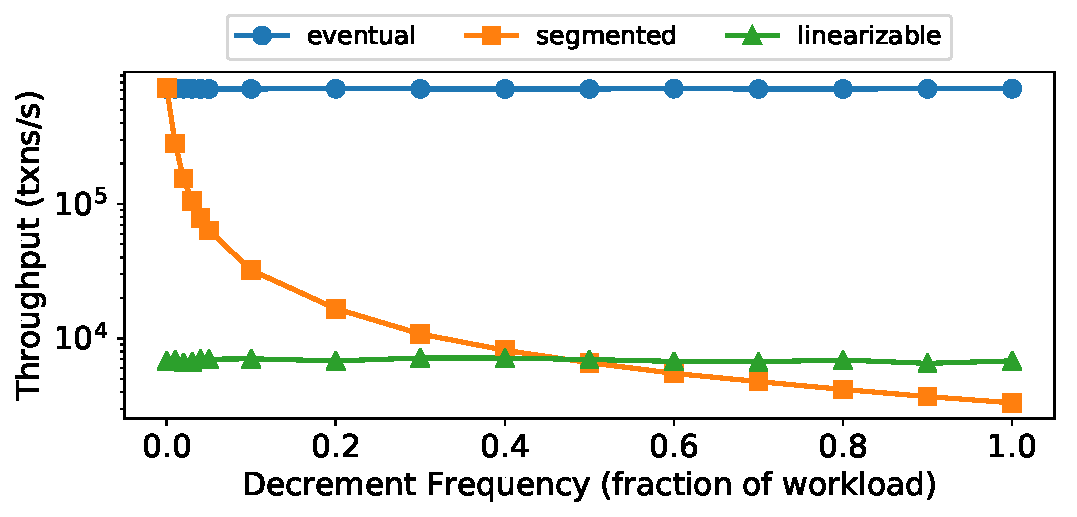
\includegraphics[width=\columnwidth]{figures/vary_withdraws.pdf}
  \end{subfigure}
  \begin{subfigure}[c]{\columnwidth}
    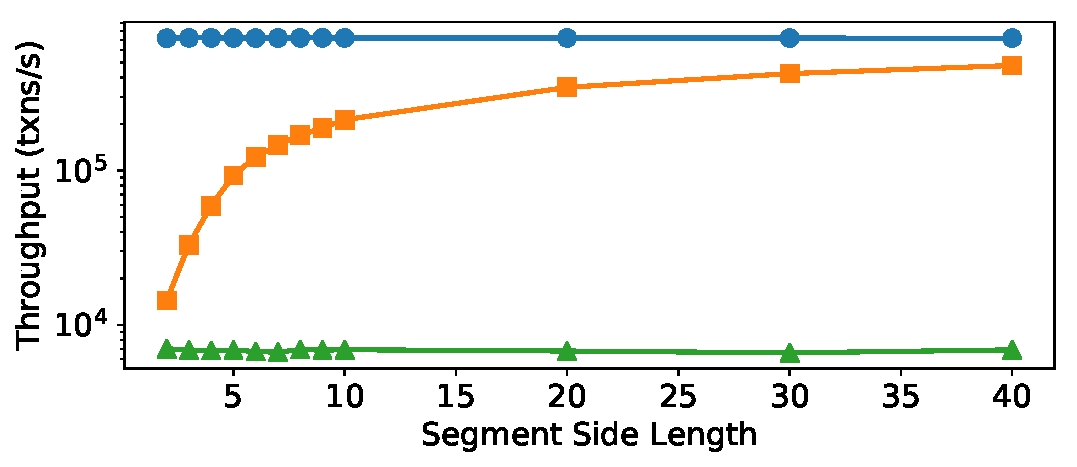
\includegraphics[width=\columnwidth]{figures/vary_segments.pdf}
  \end{subfigure}

  \caption{%
    Segmented invariant-confluent replication throughput versus coordination,
    induced by executing disallowed transactions (top) and by transitioning
    across segments (bottom).
  }\figlabel{ThroughputVsGlobalSyncs}
\end{figure}

\begin{benchmark}\benchlabel{VaryWithdraws}
Consider again the PN-Counter from \exampleref{CounreachableExample} and the
corresponding transactions, invariants, and single-segment segmentation that
forbids concurrent decrements. We replicate this object on 32 servers
deployed on 32 m5.xlarge EC2 instances within the same availability zone.  Each
server has three colocated clients that issue deposit and withdrawal
transactions. We replicate the object with eventual consistency, segmented
invariant-confluence, and linearizability and measure the system's total
throughput as we vary the fraction of client requests that are withdrawals. The
results are shown in the top of \figref{ThroughputVsGlobalSyncs}.

Both eventually consistent replication and linearizable replication are
unaffected by the workload, achieving roughly 700,000 and 7,000 transactions
per second respectively. Expectedly, eventually consistent replication
significantly outperforms linearizable replication because (a) transactions can
be sent to any server (not just the leader) and (b) servers do not coordinate
with each other at all.
%
Segmented invariant-confluent replication performs well for low-withdrawal
workloads and performs increasingly poorly as we increase the fraction of
withdrawal transactions, eventually becoming slower that linearizable
replication. For example, with 5\% withdrawal transactions, segmented
invariant-confluent replication performs an order of magnitude better than
linearizable replication; with 50\% withdrawals, it performs as well; and with
100\% withdrawals, it performs two times worse.

These results are expected. Deposit transactions can execute without any
coordination while withdrawal transactions require global coordination. As we
increase the fraction of withdrawals, we increase the amount of coordination
that the system has to perform which in turn drastically decreases the
throughput. These results also offer two insights:
%
First, for low-withdrawal workloads, segmented invariant-confluent replication
achieves a compromise between strong and weak consistency. It guarantees that
invariants are maintained (which is impossible with eventual consistency if the
object is not invariant-confluent) with performance many times better than
strongly consistent replication.
%
Second, segmented invariant-confluent replication is poorly suited to workloads
that require a large amount of coordination. For workloads without much inherit
concurrency (e.g.\ withdraw-mostly workloads), maintaining invariants is best
done with strong consistency. It provides stronger guarantees with better
performance.
\end{benchmark}

\begin{benchmark}\benchlabel{VarySegmentLength}
  Consider again the object, transactions, and invariants from \exampleref{Z2}
  and \exampleref{SegmentedZ2}. As with \benchref{VaryWithdraws}, we replicate
  the object across 32 servers. Clients issue 50\% increment $x$ transactions,
  and 50\% decrement $y$ transactions. We consider a ``checkerboard''
  segmentation $\Sigma_n = \setst{(I_{i, j}, T)}{i, j \in \ints}$ where segment
  invariant $I_{i, j}$ consists of the square of points $\setst{(x, y)}{ni \leq
  x < n(i + 1), nj \leq y < n(j + 1)}$ with side length $n$. For example,
  $\Sigma_1$ places each point in its own segment, $\Sigma_2$ tessellates
  $\ints^2$ with 2x2 squares, $\Sigma_3$ tessellates $\ints^2$ with 3x3
  squares, and so on. We measure the throughput of the object replicated with
  eventually consistent, segmented invariant-confluent, and linearizable
  replication as we vary the segment side length $n$. The results are shown in
  the bottom \figref{ThroughputVsGlobalSyncs}.

  This benchmark tells the same tale as \benchref{VaryWithdraws}. Eventual
  consistency and linearizability are unaffected by workload, and eventual
  consistency outperforms linearizability by roughly two orders of magnitude.
  In this example, the segmented invariant-confluent replication only requires
  coordination when transitioning between segment boundaries, so as we increase
  the segment side length, the throughput of the system increases
  significantly.
\end{benchmark}

\begin{figure}[ht]
  \centering
  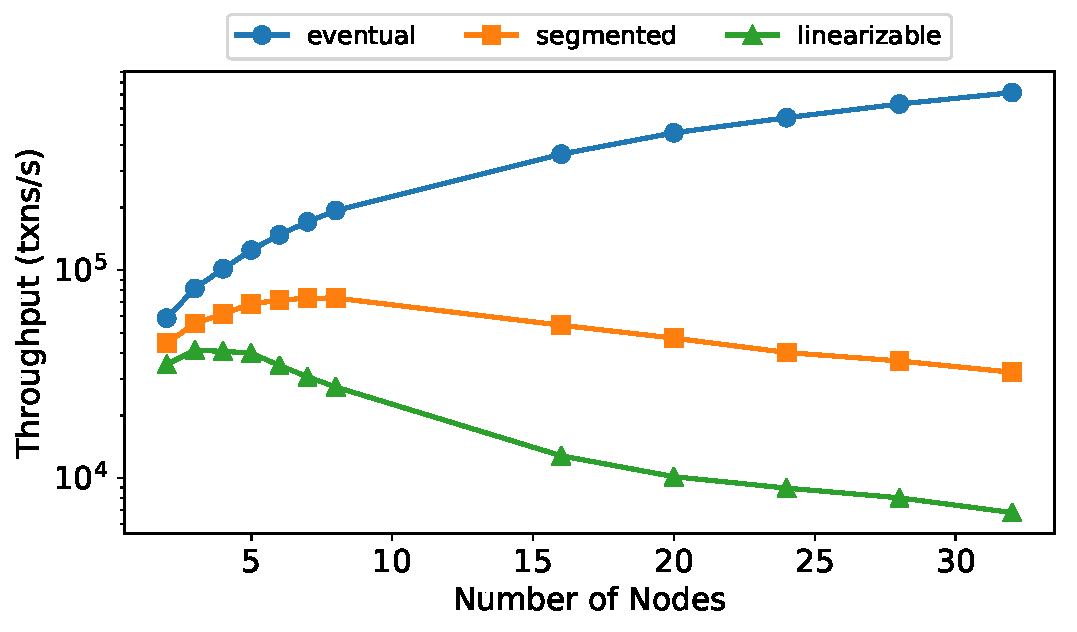
\includegraphics[width=\columnwidth]{figures/vary_nodes.pdf}
  \caption{%
    Throughput of eventually consistent, segmented invariant-confluent, and
    linearizable replication measured against the number of
    nodes.
  }\figlabel{VaryNodes}
\end{figure}

\begin{benchmark}
  In this benchmark, we measure the scale-out of segmented invariant-confluent
  replication. We repeat \benchref{VaryWithdraws} with a 10\% withdrawal rate,
  but this time we vary the number of servers we use to replicate our object.
  When we replicate with $n$ servers, we use $3n$ clients (the $3$ colocated
  clients on each server) as part of the workload. The results are shown in
  \figref{VaryNodes}.

  Eventually consistent replication scales perfectly with the number of nodes,
  confirming the results in~\cite{bailis2014coordination}. With eventually
  consistent replication, servers do not coordinate at all, so they are
  completely unaffected by the number of servers. Linearizable replication, on
  the other hand, scales up to about 3-5 servers before performance begins to
  decrease. These numbers are consistent with typical deployments of
  state-machine replication protocols like Paxos~\cite{chandra2007paxos}.
  Because all messages are sent to the leader, the leader becomes the
  bottleneck as the number of servers and clients increases. Moreover, the
  leader must wait for responses from more servers, increasing the latency of
  the slowest response which in turn decreases throughput.
  Segmented invariant-confluent replication scales up to about 6-8 servers
  before succumbing to the same scalability bottlenecks as linearizable
  replication.

  These results highlight the importance of coordination avoidance in
  distributed databases. While segmented invariant-confluent replication scales
  out slightly better than linearizable replication, both scale significantly
  worse than eventually consistent replication even for a very low (i.e.\ 10\%)
  withdrawal workload. This demonstrates that even a small amount of
  coordination can significantly reduce the scalability of a system.
\end{benchmark}
}
{\section{Related Work}
We now discuss RedBlue consistency~\cite{li2012making, li2014automating}, the
homeostasis protocol~\cite{roy2015homeostasis}, explicit
consistency~\cite{balegas2015putting}, and token-based
invariant-confluence~\cite{gotsman2016cause}: four very relevant pieces of
work. We also briefly survey other related research in the area of
invariant-confluence including program analysis in database systems, CRDTs, the
CALM theorem, and interactive proof assistants.

\newcommand{\sieve}{\textsc{sieve}}
\paragraph{RedBlue Consistency and \sieve}
RedBlue consistency is a form of consistency that sits between causal
consistency and linearizability~\cite{li2012making}. With RedBlue consistency,
every operation is labelled as red or blue. All operations are executed with
causal consistency, but with the added restrictions that red operations are
executed in a single total order embedded within the causal ordering.
RedBlue consistency is similar to segmented invariant-confluence with a single
segment in which all red operations are removed from the segment's set of
allowable transactions. In~\cite{li2012making}, Li et al.\ define
invariant safety as a sufficient condition for RedBlue consistent objects to be
invariant-confluent. Invariant safety is an analog of invariant-closure for an
operation-based (as opposed-to state based~\cite{shapiro2011conflict}) system
model. In~\cite{li2014automating}, Li et al.\ develop techniques to identify
which operations are invariant safe.  Like invariant-closure, invariant safety
is a sufficient but not necessary condition for invariant-confluence. Li et
al.\ develop sophisticated techniques for deciding invariant safety that
involve calculating weakest preconditions.  These techniques are complementary
to our work and can be used to improve the invariant-closure subroutine used by
our decision procedures.

\paragraph{The Homeostasis Protocol}
The homeostasis protocol~\cite{roy2015homeostasis} uses program analysis to
avoid unnecessary coordination between servers in a sharded database. The
protocol generates global invariants, called global treaties, and servers can
operate without coordination so long as they preserve the treaty. When the
treaty is violated, the nodes perform a round of coordination. The protocol
guarantees that transactions are executed with observational equivalence with
respect to some serial execution of the transactions. This means that
intermediate states may be inconsistent, but externally observable side effects
and the final database state are consistent. The observational equivalence
guaranteed by the homeostasis is stronger than the guarantees of
invariant-confluence. As a result, there are invariants and transaction
workloads which the homeostasis protocol would execute with more coordination
than a segmented invariant-confluent execution. Still, the homeostasis
protocol's mechanism of establishing invariants and operating without
coordination so long as the invariants are maintained is very similar to our
design of segmented invariant-confluence.

\paragraph{Explicit Consistency}
A system provides explicit consistency with respect to a partial ordering of
transactions if every server executes the transactions in a total order that
respects the partial order and in a way such that the invariant is always
preserved~\cite{balegas2015towards}. Thus, explicit consistency is like a
combination of invariant-confluence and causal consistency, similar to RedBlue
consistency. To determine if a workload is amenable to explicitly consistent
replication, Balegas et al. determine if all pairs of transactions can be
concurrently executed on the same start state without violating the invariant~\cite{balegas2015towards}.
This is a sufficient condition for explicit consistency similar to criterion
(3) in \thmref{LatticeProperty}. Balegas et al. also describe a variety of
techniques---like conflict resolution, locking, and escrow
transactions~\cite{o1986escrow}---that can be used to replicate workloads that
do meet their sufficient conditions. Conflict resolution involves choosing an
appropriate merge function; locking can be implemented as a single segment
segmentation with certain transactions disallowed; and escrow transactions can
be emulated with a segmentation that allows for concurrent decrements only when
value being decremented is sufficiently large.

\paragraph{Token-Based Invariant-Confluence}
In~\cite{gotsman2016cause}, Gotsman et al.\ discuss a hybrid token-based
consistency model that generalizes RedBlue consistency. An application designer
defines a set of tokens and specifies which pairs of tokens conflict. Then,
transactions acquire some subset of the tokens. This allows the application
designer to specify which transactions conflict at a fine granularity. With no
tokens, the model is equivalent to causal consistency. With all transactions
acquiring a single self-conflicting token, the model is equivalent to
sequential consistency~\cite{lamport1979make}. With some transactions acquiring
a single self-conflicting token and some transactions acquiring no tokens, the
model is equivalent to RedBlue consistency. Gotsman et al.\ develop sufficient
conditions to determine whether a given token scheme is sufficient to guarantee
that a global invariant is never broken. This model of consistency is very
similar to segmented invariant-confluence. The token-based approach allows
users to specify certain conflicts that are not possible with segmented
invariant-confluence. A segmentation only allows transactions within a segment
to acquire a single self-conflicting lock. However, segmented
invariant-confluence also introduces the notion of segmenting the invariant,
which cannot be emulated with the token based approach. For example,
implementing \exampleref{SegmentedZ2} with the token-based approach is
challenging without being able to segment the top-left quadrant from the
bottom-right quadrant. An interesting direction for future work is to try and
integrate the token-based approach into segmented invariant-confluence.

% Towards Fast Invariant Preservation in Geo-replicated Systems
%
% Feral
% The CISE Tool: Proving Weakly-Consistent Applications Correct
% Declarative Programming over Eventually Consistent Data Stores
% Extending Eventually Consistent Cloud Databases for Enforcing Numeric Invariants

\paragraph{Program Analysis in Database Systems}
TODO
% Program analysis in database:
%   look at some of alvins work and related stuff:
%   Find work on static partitioning of data based on program?
%   Transaction chopping / healing?

\paragraph{CRDTs}
CRDTs~\cite{shapiro2011conflict, shapiro2011comprehensive} are distributed
semilattices with inflationary update methods. Due to their algebraic
properties, CRDTs can be replicated with strong eventual consistency without
the need for any coordination. Our definition of distributed objects and our
invariant-confluence system model are inspired directly by the corresponding
definitions and system models in~\cite{shapiro2011conflict}. Note that an
invariant-confluent object does not necessarily have to be eventually
consistent. In fact, equipping a distributed object with the trivial merge
function $x \join y = x$ makes the object invariant-confluent with respect
any set of transactions and any invariant, but it makes the object very
inconsistent. Thus, it's natural (though not necessary) to use CRDTs as
invariant-confluent distributed objects, achieving a combination of eventual
consistency and invariant-preservation. Our criteria in
\thmref{LatticeProperty} also borrow ideas from CRDTs, exploiting the nice
algebraic properties of semilattices.

\paragraph{CALM Theorem}
Bloom~\cite{alvaro2010boom, alvaro2011consistency, conway2012logic} and its
formalism, Dedalus~\cite{alvaro2011dedalus, alvaro2013declarative}, are
declarative Datalog-based programming languages that are designed to program
distributed systems. The accompanying CALM
theorem~\cite{hellerstein2010declarative, ameloot2013relational} states that if
a program can be written in the monotone fragment of these languages, then
there exists a coordination-free implementation of the program. Moreover,
monotone programs are invariant to message reordering, whereas non-monotone
programs may experience anomalies if messages are reordered in the network. The
CALM theorem provides guarantees about the outputs of a program, but it does
not guarantee that invariants are maintained throughout the duration of an
execution. Moreover, Bloom and Dedalus are general purpose programming
languages that can be used to implement a variety of distributed systems (e.g.
a sharded database), while invariant-confluence is defined strictly in the
context of replicated data.

\paragraph{Proof Assistants}
Our interactive decision procedure bears resemblance to interactive proof
assistants like Coq~\cite{coq2017}, Isabelle~\cite{nipkow2002isabelle},
Agda~\cite{norell2008dependently}, and Idris~\cite{brady2013idris}. Proof
assistants guide users through the process of interactively provided a proof
that witnesses the validity of a formula. Our interactive decision procedure
guides users through the process of interactively generating a set of reachable
and unreachable points that witness the invariant-confluence of an object. An
interesting avenue for future work is to integrate an proof assistant into our
interactive decision procedure. For example, a proof assistant could verify
that a state labelled unreachable by a user is actually unreachable.
}
{\section{Conclusion}
}
{\section{Acknowledgments}
A big thanks to Alan Fekete, Peter Alvaro, Alvin Cheung, Alexandra Meliou,
Anthony Tan, and Cristina Teodoropol.
%
This research is supported in part by DHS Award HSHQDC-16-3-00083, NSF CISE
Expeditions Award CCF-1139158, and gifts from Alibaba, Amazon Web Services, Ant
Financial, CapitalOne, Ericsson, GE, Google, Huawei, Intel, IBM, Microsoft,
Scotiabank, Splunk and VMware.
}
\bibliographystyle{ACM-Reference-Format}
\bibliography{references}
\appendix
{\section{TODO}\seclabel{OriginalDefinition}
TODO
}
{\section{Operation Based Invariant Confluence}
In the system model we described, a server $p_i$ periodically sends its state
$s_i$ to some other server $p_j$ for merging. In this ``state-based'' model,
states are sent between replicas but transactions are not. Borrowing a trick
from CRDTs~\cite{shapiro2011conflict, shapiro2011comprehensive}, we can define
an alternate, but equivalent, ``operation-based'' system model in which
transactions are sent between replicas but states are not. Though the two
models are equivalent, the operation-based approach is sometimes more natural.
For example, with the operation-based approach, we can replace the PN-counter
from \exampleref{CounreachableExample} with a simple integer.

\subsection{System Model}
A \defword{distributed operation-based object} is a set $O = S$ of states. Note
that we do not have a merge function like we did with state-based objects.
%
An \defword{operation-based transaction} $t: S \to (S \to S)$ is a function
that maps a state $s$ to a \defword{shadow transaction} $t(s): S \to
S$~\cite{li2014automating}. Note that shadow transactions are curried functions
and, as we will see momentarily, can be partially applied.
%
The definition of an invariant is the same in the state-based and
operation-based models.

\begin{example}
  $\nats$ is a distributed operation-based object. $t: \nats \to (\nats \to
  \nats)$ is an operation-based transaction where $t(x)(y) = x + y$. That is,
  given a state $x$, $t(x)$ is the function $f_x$ where $f_x(y) = x + y$.
\end{example}

In our operation-based system model, a distributed object $O$ is replicated
across a set $p_1, \ldots, p_n$ of $n$ servers. Each server $p_i$ manages a
replica $s_i \in O$ of the replicated object. Every server begins with a start
state $s_0 \in S$, a fixed set $T$ of transactions, and an invariant $I$.
Servers repeatedly perform one of two actions.

First, a client can contact a server $p_i$ and request that it execute a
transaction $t \in T$. $p_i$ speculatively executes $t(s_i)$, transitioning
from state $s_i$ to state $t(s_i)(s_i)$. If $t(s_i)(s_i)$ does not satisfy the
invariant, then $p_i$ aborts the transaction and reverts to state $s_i$.
Otherwise, $p_i$ commits the transaction and remains in state $t(s_i)(s_i)$. It
also broadcasts the shadow transaction $t(s_i)$ in an exactly-once manner to
the rest of the servers.

Second, $p_j$ can receive a shadow transaction $t(s_i)$ from some other server
$p_i$. When $p_j$ receives $t(s_i)$, it transitions from its state $s_j$ to
state $t(s_i)(s_j)$. When $p_j$ receives a shadow transaction, it must execute
it, even if $\lnot I(t(s_i)(s_j))$.

Informally, $O$ is \invariantconfluent{} with respect to $s_0$, $T$, and $I$ if
every replica $s_1, \ldots, s_n$ is guaranteed to always satisfy the invariant
$I$ in every possible execution of the system.

% As with state-based objects, there are three ways to think about
% operation-based invariant-confluence: a process-based approach, a graph-based
% approach, and an expression-based approach. All three approaches are
% illustrated in \figref{OpBasedModels} and are described in more detail below.
%
% \input{figs/opbased_iconfluence.fig}
%
% \subsubsection{Process-Based}
% As with the state-based approach, the process-based model is most similar to
% the process model described by Shapiro et al.\ in~\cite{shapiro2011conflict}.
% We are given an operation-based object $O$, a start state $s_0$, a set of
% transactions $T$, an invariant $I$, and a set $\seq{p}{1}{n}$ of $n$
% processors. Each processors begins with state $s_0$. A processor $p_i$ can do
% one of two things.
%
% \begin{itemize}
%   \item
%     $p_i$ can execute a transaction $t$ on its current state $s$ and then
%     transitions from state $s$ to state $t(s)(s)$, given that $I(t(s)(s))$. If
%     $\lnot I(t(s)(s))$, then $p_i$ will not perform $t$. If $p_i$ does execute
%     $t$, then it broadcasts $t(s)$ to all other processors exactly once.
%
%   \item
%     $p_i$ can receive a broadcast shadow transaction $t(s_j)$ from some other
%     processor $p_j$. When $p_i$ receives $t(s_j)$, it transitions from its
%     state $s_i$ to state $t(s_j)(s_i)$. When $p_i$ receives a shadow
%     transaction, it must execute it, even if $\lnot I(t(s_j)(s_i))$.
% \end{itemize}
%
% $O$ is \sTIconfluent{} if every reachable state (including $s_0$) satisfies the
% invariant.
%

\subsection{Expression-Based Formalism}
To define operation-based \invariantconfluence{} formally, we represent a state
produced by an operation-based system execution as a simple expression
generated by the grammar
%
\[
  \hfill
  e ::= s \mid t(e_1)(e_2)
  \hfill
\]
%
where $s$ represents a state in $S$ and $t$ represents a transaction in $T$. As
an example, consider the system execution in \figref{OpSystemExecution} in
which a distributed object is replicated across servers $p_1$, $p_2$, and
$p_3$. Server $p_3$ begins with state $s_0$, receives transaction $t$,
transitions to state $s_1$ by executing shadow transaction $t(s_0)$,
transitions to state $s_3$ by executing shadow transaction $u(s_0)$, and then
transitions to state $s_7$ by executing shadow transaction $v(s_2)$.  In
\figref{OpExpression}, we see the abstract syntax tree of the corresponding
expression for state $s_7$.

{\begin{figure}[ht]
  \centering

  \tikzstyle{inv}=[draw=black]
  \tikzstyle{s0color}=[fill=flatred]
  \tikzstyle{s1color}=[fill=flatgreen]
  \tikzstyle{s2color}=[fill=flatdenim]
  \tikzstyle{s3color}=[fill=flatorange]
  \tikzstyle{s4color}=[fill=flatyellow]
  \tikzstyle{s5color}=[fill=flatcyan]
  \tikzstyle{s6color}=[fill=flatpurple]
  \tikzstyle{s7color}=[fill=flatblue]
  \tikzstyle{s8color}=[fill=flatdarkgray]
  \tikzstyle{txnline}=[black, thick, -latex]
  \tikzstyle{phantomstate}=[%
    shape=circle, inner sep=1pt, draw=white, line width=1pt, fill=white]
  \tikzstyle{state}=[%
    shape=circle, inner sep=1pt, draw=black, line width=1pt, text opacity=1,
    fill opacity=0.6]

  \newcommand{\internaltext}[1]{$\boldsymbol #1$}

  \begin{subfigure}[c]{0.4\textwidth}
    \centering

    \begin{tikzpicture}[xscale=1.5, yscale=1]
      \node (p3) at (0.5, 3) {$p_3$};
      \node (p2) at (0.5, 2) {$p_2$};
      \node (p1) at (0.5, 1) {$p_1$};

      \tikzstyle{pline}=[gray, opacity=0.75, thick, -latex]
      \draw[pline] (p3) to (4.5, 3);
      \draw[pline] (p2) to (4.5, 2);
      \draw[pline] (p1) to (4.5, 1);

      % Top line (phantom).
      \node[phantomstate] (s03) at (1, 3) {$\phantom{s_0}$};
      \node[phantomstate] (s13) at (2, 3) {$\phantom{s_1}$};
      \node[phantomstate] (s23) at (3, 3) {$\phantom{s_3}$};
      \node[phantomstate] (s33) at (4, 3) {$\phantom{s_6}$};

      % Middle line (phantom).
      \node[phantomstate] (s02) at (1, 2) {$\phantom{s_0}$};
      \node[phantomstate] (s12) at (2, 2) {$\phantom{s_2}$};
      \node[phantomstate] (s22) at (3, 2) {$\phantom{s_4}$};
      \node[phantomstate] (s32) at (4, 2) {$\phantom{s_7}$};

      % Bottom line (phantom).
      \node[phantomstate] (s01) at (1, 1) {$\phantom{s_0}$};
      \node[phantomstate] (s11) at (2, 1) {$\phantom{s_2}$};
      \node[phantomstate] (s21) at (3, 1) {$\phantom{s_5}$};
      \node[phantomstate] (s31) at (4, 1) {$\phantom{s_8}$};

      % Send lines.
      \tikzstyle{txntext}=[sloped, above, -latex]
      \tikzstyle{sendline}=[opacity=0.5, gray, -latex]
      \draw[txnline, sendline] (s03) to (s22);
      \draw[txnline, sendline] (s03) to (s31);
      \draw[txnline, sendline] (s02) to (s23);
      \draw[txnline, sendline] (s02) to (s11);
      \draw[txnline, sendline] (s11) to (s33);
      \draw[txnline, sendline] (s11) to (s32);

      % Top line.
      \node[state, s0color] (s03) at (1, 3) {\internaltext{s_0}};
      \node[state, s1color] (s13) at (2, 3) {\internaltext{s_1}};
      \node[state, s3color] (s23) at (3, 3) {\internaltext{s_3}};
      \node[state, s6color] (s33) at (4, 3) {\internaltext{s_6}};

      % Middle line.
      \node[state, s0color] (s02) at (1, 2) {\internaltext{s_0}};
      \node[state, s2color] (s12) at (2, 2) {\internaltext{s_2}};
      \node[state, s4color] (s22) at (3, 2) {\internaltext{s_4}};
      \node[state, s7color] (s32) at (4, 2) {\internaltext{s_7}};

      % Bottom line.
      \node[state, s0color] (s01) at (1, 1) {\internaltext{s_0}};
      \node[state, s2color] (s11) at (2, 1) {\internaltext{s_2}};
      \node[state, s5color] (s21) at (3, 1) {\internaltext{s_5}};
      \node[state, s8color] (s31) at (4, 1) {\internaltext{s_8}};

      % Transaction lines.
      \draw[txnline] (s03) to node[txntext]{$t(s_0)$} (s13);
      \draw[txnline] (s02) to node[txntext]{$u(s_0)$} (s12);
      \draw[txnline] (s11) to node[txntext]{$v(s_2)$} (s21);
      \draw[txnline] (s13) to node[txntext]{$u(s_0)$} (s23);
      \draw[txnline] (s23) to node[txntext]{$v(s_2)$} (s33);
      \draw[txnline] (s12) to node[txntext]{$t(s_0)$} (s22);
      \draw[txnline] (s22) to node[txntext]{$v(s_2)$} (s32);
      \draw[txnline] (s01) to node[txntext]{$u(s_0)$} (s11);
      \draw[txnline] (s21) to node[txntext]{$t(s_2)$} (s31);
    \end{tikzpicture}

    \caption{System Execution}\figlabel{OpSystemExecution}
  \end{subfigure}

  \begin{subfigure}[c]{0.3\textwidth}
    \centering

    \begin{tikzpicture}[xscale=0.75]
                         \node[state, s7color, label={[label distance=-0.1cm] 90:$s_7$}] (s7) at (0, 0) {\internaltext{v}};
      \draw (s7)++(210:1) node[state, s2color, label={[label distance=-0.1cm] 90:$s_2$}] (s2)           {\internaltext{u}};
      \draw (s7)++(-30:1) node[state, s4color, label={[label distance=-0.1cm] 90:$s_4$}] (s4)           {\internaltext{t}};
      \draw (s2)++(210:1) node[state, s0color]                                           (n1)           {\internaltext{s_0}};
      \draw (s2)++(-90:1) node[state, s0color]                                           (n2)           {\internaltext{s_0}};
      \draw (s4)++(225:1) node[state, s0color]                                           (n3)           {\internaltext{s_0}};
      \draw (s4)++(-45:1) node[state, s2color, label={[label distance=-0.1cm] 90:$s_2$}] (s22)          {\internaltext{u}};
      \draw (s22)++(225:1) node[state, s0color]                                          (n4)           {\internaltext{s_0}};
      \draw (s22)++(-45:1) node[state, s0color]                                          (n5)           {\internaltext{s_0}};

      \tikzstyle{astedge}=[thick]
      \draw[astedge] (s7) to (s2) to (n1);
      \draw[astedge] (s7) to (s2) to (n2);
      \draw[astedge] (s7) to (s4) to (n3);
      \draw[astedge] (s7) to (s4) to (s22) to (n4);
      \draw[astedge] (s7) to (s4) to (s22) to (n5);
    \end{tikzpicture}

    \caption{Expression}\figlabel{OpExpression}
  \end{subfigure}

  \caption{An operation-based system execution and corresponding expression}
  \figlabel{OpDefinitions}
\end{figure}
}

We say an expression $e$ is \defword{\sTIreachable{}} if it corresponds to a
valid execution of our system model. Formally, we define
$\sTIreachablepredicate{e}$ to be the smallest predicate that satisfies the
following equations:
\begin{itemize}
  \item
    $\sTIreachablepredicate{s_0}$.
  \item
    For all expressions $e_1, e_2$ and for all transactions $t$ in $T$, if
    $\sTIreachablepredicate{e_1}$, $\sTIreachablepredicate{e_2}$, and
    $I(t(e_1)(e_1))$, then $\sTIreachablepredicate{t(e_1)(e_2)}$.
\end{itemize}

Finally, we say $O$ is \invariantconfluent{} with respect to $s_0$, $T$, and
$I$, abbreviated \sTIconfluent{}, if all reachable states satisfy the
invariant:
\[
  \hfill
  \setst{s \in S}{\sTIreachablepredicate{s}} \subseteq I
  \hfill
\]
}
\end{document}
